\section{Implementation}

This section starts by describing some important algorithms and implementation details of Atmosphere.

\subsection{Classes, data structures and algorithms}


This subsection describes data structures and algorithms used in JavaScript implementation. At the time of writing, the Cocoa implementation does not include all of the functionality described here.

\subsubsection{Data structures}

\textbf{URI} is a structure (in JavaScript implemented as object) which represents unique address of a local object. It consists of \textbf{entity} and \textbf{identifier}.

\textbf{Meta object} is structure which represents the meta information for an object. It contains the link back to the original object in the application store, and the values of meta attributes. Every application object managed by Atmosphere is assigned a meta object.

\subsubsection{Classes overview}

Both implementations provide object-oriented system of code organization. Components of Atmosphere are represented using classes as pictured in Figure \ref{fig:1}.

\begin{figure}[ht!]
\centering
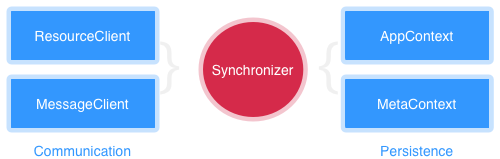
\includegraphics[width=350pt]{GeneralImplementation.png}
\caption{Classes used in implementation of Atmosphere \label{fig:1}}
\end{figure}


\subsubsection{Synchronizer}

Synchronizer is the main class of Atmosphere. It lies on top of other classes, and other classes use it to accomplish tasks. Its method can be divided into following groups.

\begin{enumerate}
\item Object lifecycle
\item Updating local objects with new data
\item Fetching objects
\item Saving objects
\item Making custom REST requests
\item Marking object as changed or synchronized
\item Synchronization
\end{enumerate}

\textbf{Object lifecycle} consists of class constructor, which initializes the class and all other required classes.

\textbf{Updating local objects} provides method for updating object specified by URI with new data. It also checks if updating data would change identifier of object, if so, then it updates the identifier in both application and meta context.

\textbf{Fetching objects} and \textbf{making custom REST requests} forward the call to resource client. These are only convenience methods. Similarly, \textbf{marking object as changed or synchronized} methods are forwarded to the meta context.

\textbf{Saving objects} allows specifying option which would make the saving 'synchronous'. In such case Atmosphere will immediately produce a save network request. When this option is set to false, the object is only marked as changed, and is synchronized in the next synchronization loop.

There are two purposes for this option: First, it disables offline usage. If the request fails, it will not be attempted again. Second, it is possible to pass options to such request. Note that asynchronous saving doesn't allow any options to be sent along with the save method. Making saving synchronous enables extra options, such as URL arguments or extra POST body.

\textbf{Synchronization} contains logic for looking up changed objects in meta context, deciding whether to send a create or update request, and finally calling the save method of resource client.

\subsubsection{Communication}

The communication layer consists of two classes: The resource client and the message client.

\textbf{Resource client} is used to download data over HTTP protocol conforming to REST style. In order to make a HTTP request, we need a URL for the resource. The process of converting a model and action pair to URL string is called routing. It is done by specifying an application specific routing table similar to one pictured in Figure \ref{fig:Routing}.

\begin{figure}[htbp]
  \centering
    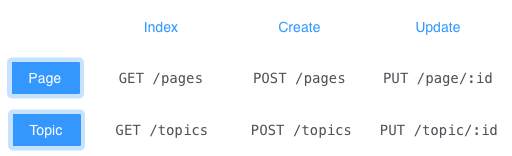
\includegraphics[width=300pt]{Routing.png}
  \caption{Example routing table for resource client}
  \label{fig:Routing}
\end{figure}

Once the correct URL is looked up in the table, the resource client prepends the base URL for the REST source, replaces occurrences of ID string with ID of record being saved, processes extra request-specific options and sends the request.

Resource client is also responsible for extracting data contained in the response returned from HTTP call. In the current implementation, only the JSON format is supported. Since the response could store data in many different ways (see Listing \ref{json}), Atmosphere allows setting custom function (or block in Objective-C) for retrieving these data from the JSON response.

\begin{lstlisting}[caption=Different formats of response JSON data,label=json]
// Simple JSON response
[{name: "Edukit"}, {name: "Atmosphere"}]
// More complicated JSON response
{"projects": [{"project": {name: "Edukit"}}, {"project": {name: "Atmosphere"}}]}
\end{lstlisting}

\textbf{Message client} is responsible for opening and maintaining connection over WebSocket. Both JavaScript and Cocoa implementations use Socket.IO \citep{socketio}, a pseudo-protocol implemented on top of WebSocket.

The typical update message contains object identifier and its data. The message client is responsible for updating the object with data contained in the message and it does so by calling appropriate method in the synchronizer class. Therefore message client remains a very lightweight class.

\subsubsection{Persistence}

\textbf{Application context} is class that manages application objects by providing methods such as create, update, change identifier or delete.

It's job is to unify interfaces of different model layers where Atmosphere might be used. In the current version, the only model layer is the one of Spine framework, but this class provides portability to other environments by encapsulating framework-specific model-related code.

\textbf{Meta context} manages meta information for each of application objects. It provides methods for finding meta objects for existing application objects, creating new ones, changing identifiers and updating meta attributes.

The motivation for this class came from the original implementation of Atmosphere which was intended only for Cocoa applications. Cocoa uses SQLite to store application objects, so it is not possible to dynamically add attributes to the schema.

Atmosphere needs some extra attributes, such as 'is changed' or 'is local only'. Therefore a new schema is used, where each item contains identifier of the application object and values for these meta attributes.

\subsection{JavaScript details}

At the time of writing, JavaScript implementation of Atmosphere is built on top of the Spine \citep{spinejs} library which is a lightweight framework for building JavaScript web applications.

The library doesn’t completely rely on Spine, instead it only utilizes its model layer. Furthermore, all the code that requires Spine is contained in one small file (application context), which can be easily rewritten for other client side frameworks and their own model layers.

The implementation is written in CoffeeScript \citep{coffeescript}, which is a language that improves syntax of JavaScript by introducing many syntactic shortcuts such as semantic whitespace (inspired by Python) or accessing instance variables with the '@' sign. (inspired by Ruby).

The classes in persistence and communication layers implement the basic roles of Atmosphere, while the Synchronizer class is the entry point for working with Atmosphere.

The Spine integration contains shortcuts for calling Atmosphere methods directly from Spine models using the API users are already developers are already familiar with.

JavaScript implementation uses Socket.IO \citep{socketio} client library for opening WebSocket connections. The library enables socket-like functionality in browsers that don't support WebSocket using long-polling or Adobe Flash.

\subsection{Cocoa details}

The Cocoa implementation is packaged as Xcode framework. It is written in Objective-C and can be compiled for both desktop (Mac) and mobile (iPhone and iPad) platforms.

The Cocoa implementation relies on Core Data which is standard for storing objects in Cocoa applications. It binds onto Core Data workflow which allows automatically saving objects remotely as they are saved in the local store.